\documentclass{article}
\usepackage{float}
\usepackage{arxiv}
\usepackage{graphicx}
\usepackage[utf8]{inputenc} % allow utf-8 input
\usepackage[T1]{fontenc}    % use 8-bit T1 fonts
%\usepackage{hyperref}       % hyperlinks
\usepackage{url}            % simple URL typesetting
\usepackage{booktabs}       % professional-quality tables
\usepackage{amsfonts}       % blackboard math symbols
\usepackage{amsmath}        % for \eqref and advanced math environments
\usepackage{nicefrac}       % compact symbols for 1/2, etc.
\usepackage{microtype}      % microtypography
\usepackage{lipsum}
\usepackage[colorlinks=true, allcolors=black]{hyperref}
\usepackage{subcaption}

%\usepackage[hidelinks]{hyperref}


\title{
\huge \textit{Parallel Programming Course — Final Project Proposal} \\\Large \textit{Topic:Ultrasound Synthetic Aperture Beamforming Acceleration}
\\\Large \textit{Group-22}
}


\author{
Cheng-Po, Chi \\
r12945010
\And
Chin-Hui,Chu \\
r12944041
\And
Yi-Hua, Chuang \\
b10201029
}


%\author{group-22} \\

  %% \And
  %% Coauthor \\
  %% Affiliation \\
  %% Address \\
  %% \texttt{email} \\
  %% \And
  %% Coauthor \\
  %% Affiliation \\
  %% Address \\
  %% \texttt{email} \\
\date{}
\begin{document}
\maketitle


\section{Introduction}

Ultrasound beamforming is the core signal-processing technique in array-based ultrasound imaging systems. 
Its primary purpose is to temporally align (delay alignment) the echo signals received by each array element of the transducer, so that the spatial energy distribution can be accurately reconstructed and presented as an interpretable image. 
Among existing approaches, Delay-and-Sum (DAS) beamforming is the most fundamental and widely adopted method. 
After applying the appropriate time delays, DAS sums the signals received across all channels to produce the final beamformed output. 


\begin{figure}[H]
    \centering
    % 第一張子圖
    \begin{subfigure}[b]{0.6\linewidth}
        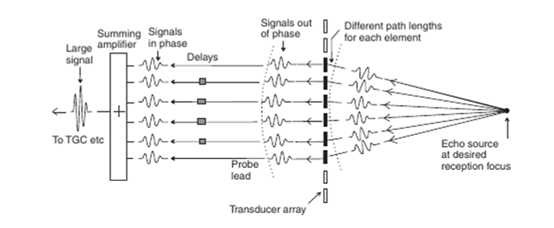
\includegraphics[width=\linewidth]{圖片1.png}
        \caption{Concept of delay-and-sum~\cite{asl2024beamforming}}
        \label{fig:sub1}
    \end{subfigure}
    \hfill
    % 第二張子圖
    \begin{subfigure}[b]{0.35\linewidth}
        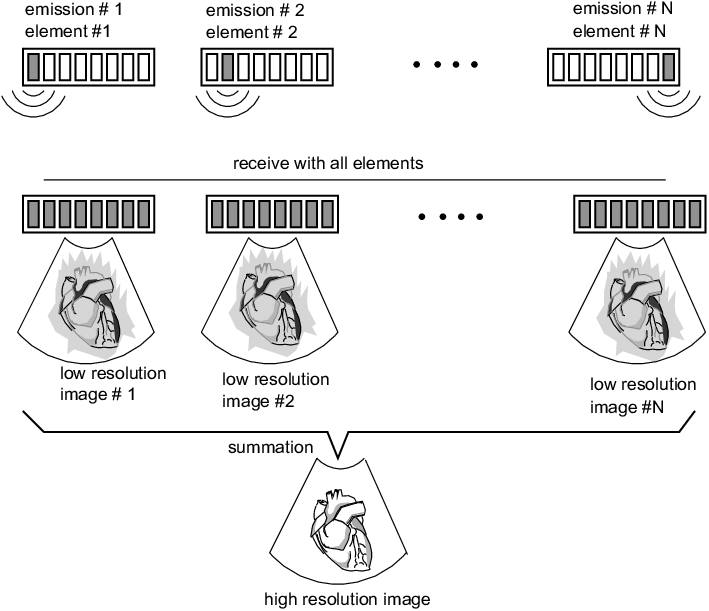
\includegraphics[width=\linewidth]{Basic-principle-of-synthetic-aperture-ultrasound-imaging-from-9.png}
        \caption{Concept of sythetic aperture~\cite{inproceedings}}
        \label{fig:sub2}
    \end{subfigure}
    
    \caption{}
    \label{fig:all}
\end{figure}
As shown in Fig.~\ref{fig:sub1}, when an ultrasound signal originates from a point in space, each array element receives the echo at a different time due to its varying distance from that point. 
Consequently, the received signals are misaligned in time and cannot accurately represent the true location or amplitude of that point. 
By applying the appropriate time delays to each channel, the signals can be aligned along the time axis; summing the aligned signals then yields the correct beamformed response. 

Furthermore, to overcome the resolution limitations imposed by the physical size of the transducer when using a conventional fixed transmit aperture, \textbf{Synthetic Aperture Imaging (SA)} has been introduced as an important technique for improving imaging performance. 
In SA, each transmission uses only a subset of array elements as the transmit aperture, while the full array is used for reception.
Through multiple independent transmissions, the system accumulates several sets of sub-aperture data over time. 
After applying appropriate delay compensation and coherent summation, these data effectively enlarge the equivalent aperture, thereby enhancing lateral resolution(Fig.~\ref{fig:sub2}). 
Despite these benefits, SA processing introduces substantial computational complexity, which is discussed in the following sections.

% ======================================================
% Synthetic Aperture Beamforming (SA) Explanation
% ======================================================

In synthetic aperture (SA) ultrasound imaging, the final image value at each spatial location is formed by coherently combining time-delayed echo signals acquired from multiple transmit--receive element pairs. 
Let $\mathbf{r}$ denote the spatial coordinate of the pixel of interest (e.g., $(x,z)$ or $(r,\theta)$). 
Assume an array with $N$ elements; the position of the $i$-th element is denoted by $\mathbf{r}_i$. 
The medium sound speed is $c$. 
For a pixel at location $\mathbf{r}$, when the $p$-th element is used as the transmitter and the $n$-th element as the receiver, the total acoustic round-trip delay is given by
\begin{equation}
\tau_{p,n}(\mathbf{r})
    = \frac{\|\mathbf{r} - \mathbf{r}_p\| + \|\mathbf{r} - \mathbf{r}_n\|}{c}.
\label{eq:SA_delay}
\end{equation}

The received RF data are sampled at a frequency $f_s$. 
Thus, the continuous-time delay $\tau_{p,n}(\mathbf{r})$ corresponds to the discrete sample index
\begin{equation}
k_{p,n}(\mathbf{r}) 
    = \mathrm{round}\!\left(\tau_{p,n}(\mathbf{r})\, f_s\right).
\label{eq:SA_index}
\end{equation}

The delay-compensated RF sample corresponding to pixel $\mathbf{r}$ is obtained by directly indexing the RF signal:
\begin{equation}
\tilde{s}_{p,n}(\mathbf{r})
    = s_{p,n}\!\left[k_{p,n}(\mathbf{r})\right],
\label{eq:SA_sample}
\end{equation}
where $s_{p,n}[k]$ denotes the $k$-th discrete RF sample acquired from the $n$-th receive element after the $p$-th transmit event.

Finally, the beamformed output at pixel $\mathbf{r}$ is produced by coherently summing all transmit--receive combinations:
\begin{equation}
y(\mathbf{r})
    = \sum_{p=1}^{N} \sum_{n=1}^{N} 
        w_{p,n}(\mathbf{r}) \, \tilde{s}_{p,n}(\mathbf{r}),
\label{eq:SA_sum}
\end{equation}
where $w_{p,n}(\mathbf{r})$ denotes an apodization weight applied to control the effective aperture and suppress sidelobes. 
Equations~\ref{eq:SA_delay}--\ref{eq:SA_sum} together define the synthetic aperture beamforming process based on discrete delay compensation and coherent combination.

These operations constitute the primary computational workload of SA imaging and directly lead to the challenges described in the next section.

% ======================================================
% Motivation
% ======================================================

\section{Motivation}

Synthetic aperture (SA) beamforming offers improved lateral resolution by coherently combining echo signals from all transmit--receive element pairs. 
However, this enhanced image quality comes at the cost of extremely high computational complexity. 
For an array with $N$ elements, SA reconstruction requires processing $N^2$ transmit--receive paths for every image pixel. 
Moreover, each path involves computing the round-trip delay, converting it to a discrete sample index, and extracting the corresponding RF value. 
When performed over a two-dimensional image grid, the total number of delay-and-sample operations becomes prohibitively large. 

In practical ultrasound systems, real-time imaging demands frame rates on the order of thirty frames per second. 
The computational burden of SA beamforming therefore becomes the primary bottleneck limiting its deployment in real-time applications on conventional CPU-based systems. 
Recent advances in massively parallel hardware platforms, especially graphics processing units (GPUs), provide an effective solution for accelerating SA reconstruction. 
The delay computation, RF sample indexing, and pixel-wise coherent summation are inherently parallelizable, making SA beamforming an ideal candidate for GPU acceleration.

Thus, the motivation of this work is to leverage GPU parallel computing to overcome the computational bottleneck of SA imaging, enabling high-resolution synthetic aperture ultrasound reconstruction with near real-time performance.

% ======================================================
% Target Topic
% ======================================================

\section{Target Topic}


To accelerate SA beamforming on GPUs, a straightforward parallelization strategy is to assign one thread to each image pixel. 
Under this pixel-based scheme, every thread must compute the delay for all $N^2$ transmit--receive element pairs, convert each delay into a sample index, and then access the corresponding RF data. 
However, this implies that each thread must repeatedly access the entire RF dataset, which often occupies several megabytes of global memory and results in extremely high memory traffic.

For example, consider a typical SA configuration with $N=128$ array elements and $2048$ samples per receive channel. 
The total size of the RF dataset is
\[
128 \times 128 \times 2048 \times 2~\text{bytes}
= 67,108,864~\text{bytes} \approx 64~\text{MB},
\]
assuming 16-bit sampled RF data. 
During pixel-based processing, every thread must repeatedly read from this $\approx 64$ MB dataset, which far exceeds the effective global-memory bandwidth available per thread. 
As a result, the computation becomes memory-bound, and the GPU is unable to reach its theoretical compute throughput.

Moreover, the $N^2$ delay paths associated with each pixel offer little opportunity for data reuse across threads. 
This leads to redundant memory loads and further limits the achievable memory bandwidth. 
Consequently, naive pixel-based parallelization generally fails to exploit the massive parallelism of the GPU, motivating the need for more efficient parallelization strategies and memory-access patterns that better match the characteristics of SA beamforming.

In this work, real ultrasound RF data acquired from an actual imaging system are used as the test case. 
The output generated by the serial CPU implementation serves as the ground truth reference for validating the correctness of the GPU-accelerated SA reconstruction.





\section{Schedule}
\begin{table}[h]
    \centering
    \begin{tabular}{|l|l|}
        \hline
        Date & Objective\\\hline
        11/16 & Completion of final project proposal\\\hline
        11/17 -- 11/23 & Literature review and related work survey\\\hline
        11/24 -- 12/07 & Exploration and testing of alternative parallelization strategies\\\hline
        12/07 -- 12/12 & Ablation studies and refinement of the selected approach\\\hline
        12/14 -- 12/19 & Preparation of final presentation materials\\\hline
        12/19 & Final project presentation\\\hline
    \end{tabular}
\end{table}

\section{Implementation plans}

We currently have a working serial CPU implementation of the SA beamformer, which requires about two minutes to reconstruct a single frame. Our goal is to port this implementation to the GPU and apply parallelization and memory-optimization techniques to reduce the runtime to approximately $3\times 10^{-2}$ seconds. Achieving this speed would transform the system from non-interactive processing to real-time performance, providing a dramatically better user experience.

First, the existing CPU implementation will be preserved as a correctness and performance baseline. The GPU output will be validated against this reference.

Next, we will design a GPU version based on a tile-based parallelization strategy. The output image will be divided into small two-dimensional tiles, each processed by a CUDA thread block. Threads within a block will collaboratively handle the pixels in the tile and iterate over all required transmit--receive pairs. We will also consider partitioning RF data into subsets so that tiles can be further distributed across multiple blocks if needed.

To improve memory efficiency, we will leverage the GPU memory hierarchy. RF data will be accessed in a coalesced manner and cached in shared memory to reduce global-memory traffic, while static parameters such as element positions and apodization weights will be placed in constant memory. We will tune block size, thread layout, and per-thread pixel workload to balance register usage and occupancy and better hide memory latency.

Finally, we will profile the GPU kernels and conduct a brief ablation study comparing different tile sizes, thread mappings, and shared-memory strategies. The configuration offering the highest speedup with acceptable reconstruction error will be selected as the final implementation.


\bibliographystyle{unsrt}  

\bibliography{REFERENCES}  




\end{document}
